% Stereographic (half-angle) coordinate from P0 = (-1,0) = (6,0).
% t = sin k / (1 + cos k); P0 itself is t = infinity.
\documentclass[tikz,border=8pt]{standalone}
\usepackage{amsmath,amssymb}
\begin{document}
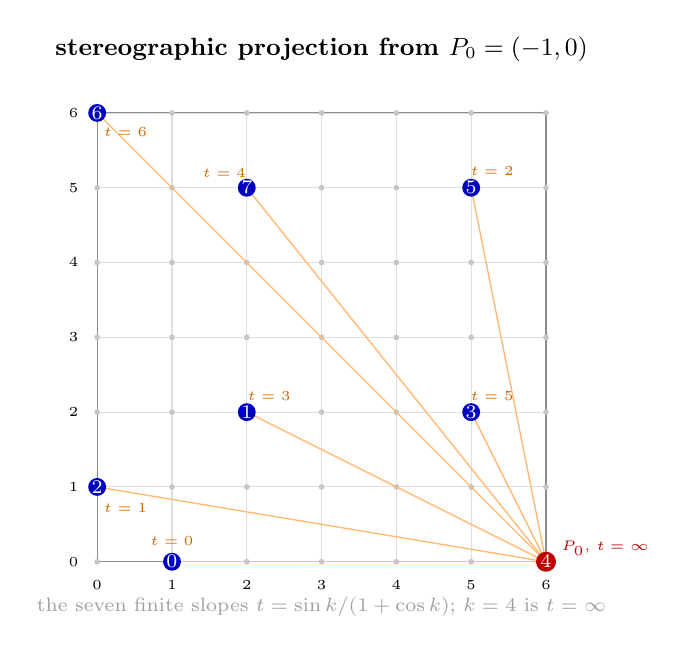
\begin{tikzpicture}[scale=0.95]
  \draw[gray!25] (0,0) grid (6,6);
  \draw[black!45] (0,0) rectangle (6,6);
  \foreach \x in {0,...,6} {%
    \foreach \y in {0,...,6} \fill[gray!45] (\x,\y) circle (1.1pt);}
  \foreach \x in {0,...,6} \node[font=\tiny,below] at (\x,-0.12) {\x};
  \foreach \y in {0,...,6} \node[font=\tiny,left] at (-0.12,\y) {\y};
  % projection lines from P0
  \foreach \x/\y in {1/0,2/2,0/1,5/2,5/5,0/6,2/5} {%
    \draw[orange!55, line width=0.5pt] (6,0)--(\x,\y);}
  % the eight points
  \foreach \x/\y/\k in {1/0/0,2/2/1,0/1/2,5/2/3,5/5/5,0/6/6,2/5/7} {%
    \fill[blue!75!black] (\x,\y) circle (3.4pt);
    \node[font=\scriptsize,text=white] at (\x,\y) {\k};}
  \fill[red!75!black] (6,0) circle (3.8pt);
  \node[font=\scriptsize,text=white] at (6,0) {$4$};
  % t labels
  \node[font=\tiny,text=orange!80!black] at (1.0,0.28) {$t=0$};
  \node[font=\tiny,text=orange!80!black] at (0.38,0.72) {$t=1$};
  \node[font=\tiny,text=orange!80!black] at (2.30,2.22) {$t=3$};
  \node[font=\tiny,text=orange!80!black] at (5.28,2.22) {$t=5$};
  \node[font=\tiny,text=orange!80!black] at (5.28,5.22) {$t=2$};
  \node[font=\tiny,text=orange!80!black] at (1.70,5.20) {$t=4$};
  \node[font=\tiny,text=orange!80!black] at (0.38,5.75) {$t=6$};
  \node[font=\tiny,text=red!75!black,anchor=west] at (6.08,0.18) {$P_0$, $t=\infty$};
  \node[font=\small\bfseries] at (3,6.85) {stereographic projection from $P_0=(-1,0)$};
  \node[font=\scriptsize,gray!75] at (3,-0.6)
    {the seven finite slopes $t=\sin k/(1+\cos k)$; $k=4$ is $t=\infty$};
\end{tikzpicture}
\end{document}
